\input{preambulo_presentacion_Berlin_beaver}
\usepackage{pifont}
\usepackage{siunitx}
\usetikzlibrary{shapes}
\newcommand{\cmark}{\ding{51}}%
\newcommand{\xmark}{\ding{55}}%
\definecolor{cadmiumgreen}{rgb}{0.0, 0.42, 0.24}
\makeatletter
\setbeamertemplate{footline}
{
  \leavevmode%
  \hbox{%
  \begin{beamercolorbox}[wd=.333333\paperwidth,ht=2.25ex,dp=1ex,center]{section in foot}%
    \usebeamerfont{section in foot} \insertsection
  \end{beamercolorbox}%
  \begin{beamercolorbox}[wd=.333333\paperwidth,ht=2.25ex,dp=1ex,center]{subsection in foot}%
    \usebeamerfont{subsection in foot}  \insertsubsection
  \end{beamercolorbox}%
  \begin{beamercolorbox}[wd=.333333\paperwidth,ht=2.25ex,dp=1ex,right]{date in head/foot}%
    \usebeamerfont{date in head/foot} \insertshortdate{} \hspace*{2em}
    \insertframenumber{} / \inserttotalframenumber \hspace*{2ex} 
  \end{beamercolorbox}}%
  \vskip0pt%
}
\makeatother
%--------------------------------------------------------------------
%--------------------------------------------------------------------
\newcounter{choice}
\renewcommand\thechoice{\Alph{choice})}
%\newcommand\choicelabel{\thechoice.}
\newcommand\choicelabel{\thechoice}

\newenvironment{choices}%
  {\list{\choicelabel}%
     {\usecounter{choice}\def\makelabel##1{\hss\llap{##1}}%
       \settowidth{\leftmargin}{W.\hskip\labelsep\hskip 2.5em}%
       \def\choice{%
         \item
       } % choice
       \labelwidth\leftmargin\advance\labelwidth-\labelsep
       \topsep=0pt
       \partopsep=0pt
     }%
  }%
  {\endlist}

\newenvironment{oneparchoices}%
  {%
    \setcounter{choice}{0}%
    \def\choice{%
      \refstepcounter{choice}%
      \ifnum\value{choice}>1\relax
        \penalty -50\hskip 1em plus 1em\relax
      \fi
      \choicelabel
      \nobreak\enskip
    }% choice
    % If we're continuing the paragraph containing the question,
    % then leave a bit of space before the first choice:
    \ifvmode\else\enskip\fi
    \ignorespaces
  }%
  {}
%----------------------------------------------------------
%----------------------------------------------------------

\setbeamertemplate{navigation symbols}{}
\date{20 de marzo de 2021}
\title{Sesión 5. Matemáticas}
\subtitle{Asesoría}
\begin{document}
\maketitle
\fontsize{14}{14}\selectfont
\spanishdecimal{.}
\section*{Contenido}
\frame[allowframebreaks]{\tableofcontents[currentsection, hideallsubsections]}
\section{Fracciones}
\frame{\tableofcontents[currentsection, hideothersubsections]}

\subsection{Conceptos}

\begin{frame}
\frametitle{Conceptos}
Una \textcolor{red}{Fracción} es un par ordenado de números enteros.
\\
\bigskip
\pause
Una fracción se representa mediante un \emph{numerador} y un \emph{denominador}.
\begin{align*}
\dfrac{3}{5}
\end{align*}
\begin{figure}[H]
\begin{tikzpicture}[overlay]
    \draw [thick, ->] (-2, 2) -- (-0.5, 2);
    \node [text = blue] at (-3, 1.8) {Numerador};
    \draw [thick, <-] (0.5, 1.5) -- (2, 1.5);
    \node [text = blue] at (2.5, 1.1) {Denominador};
\end{tikzpicture}
\end{figure}
\end{frame}
\begin{frame}
\frametitle{Las fracciones}
Una fracción cuyo numerador y denominador son iguales, representa la unidad.
\begin{eqnarray*}
\dfrac{5}{5} = 1 \\[0.5em] \pause
\dfrac{11}{11} = 1 \\[0.5em] \pause
\dfrac{2}{2} = 1 \\[0.5em] \pause
\dfrac{124}{124} = 1
\end{eqnarray*}
\end{frame}
\begin{frame}
\frametitle{Fracción propia}
Una fracción \textcolor{blue}{propia}, es aquella cuando el valor de la fracción es menor que la unidad.
\begin{align*}
\dfrac{3}{5}, \hspace{0.5cm} \dfrac{1}{7}, \hspace{0.5cm} \dfrac{23}{100}
\end{align*}
\pause
Otra manera de ver a una fracción propia, es que el numerador es menor que el denominador.
\end{frame}
\begin{frame}
\frametitle{Fracción impropia}
Una fracción \textcolor{red}{impropia}, es aquella cuando el valor de la fracción es mayor que la unidad:
\begin{align*}
\dfrac{4}{3}, \hspace{0.5cm} \dfrac{10}{7}, \hspace{0.5cm} \dfrac{23}{15}
\end{align*}
\pause
Aquí reconocemos que el numerador es mayor que el denominador.
\end{frame}
\begin{frame}
\frametitle{Fracciones homogéneas}
Dos o más fracciones, que tiene igual denominador se llaman \textcolor{brown}{homogéneas}:
\begin{align*}
\dfrac{1}{4}, \hspace{0.5cm} \dfrac{7}{4}, \hspace{0.5cm} \dfrac{10}{4}
\end{align*}
\pause
Si tienen distinto denominador se llaman \textcolor{brown}{heterogéneas}.
\begin{align*}
\dfrac{3}{4}, \hspace{0.5cm} \dfrac{1}{5}, \hspace{0.5cm} \dfrac{11}{13}
\end{align*}
\end{frame}
\begin{frame}
\frametitle{Fracciones inversas}
Dos fracciones son \textcolor{blue}{inversas}, si el numerador de una, es denominador de la otra y viceversa.
\begin{align*}
\dfrac{5}{4}, \hspace{0.5cm} \dfrac{4}{5}
\end{align*}
\end{frame}
\begin{frame}
\frametitle{Fracciones equivalentes}
Dos fracciones son \textcolor{red}{equivalentes} si representan una misma cantidad, aunque el numerador y el denominador sean diferentes:
\begin{align*}
\dfrac{1}{2}, \hspace{0.5cm} \dfrac{2}{4}
\end{align*}
\begin{tikzpicture}[overlay]
    \draw (4, -1) rectangle (5, 0);
    \draw [fill=gray, opacity=0.5] (4, -1) rectangle (4.5, 0);
    \draw (6, -1) rectangle (7, 0);
    \draw [fill=gray, opacity=0.5] (6, -1) rectangle (6.5, 0);
    \draw (6, -0.5) -- (7, -0.5);
\end{tikzpicture}
\end{frame}
\begin{frame}
\frametitle{Fracción reductible}
Una fracción es \textcolor{purple}{reductible}, cuando sus términos tienen más de un divisor común:
\begin{align*}
\dfrac{4}{6}, \hspace{0.5cm} \dfrac{25}{50}, \hspace{0.5cm} \dfrac{100}{360}
\end{align*}
\end{frame}
\begin{frame}
\frametitle{Fracción irreductible}
Una fracción es \textcolor{orange}{irreductible}, si el numerador y el denominador son primos entre sí.
\begin{align*}
\dfrac{1}{3}, \hspace{0.5cm} \dfrac{7}{9}, \hspace{0.5cm} \dfrac{13}{15}
\end{align*}
\pause
Recordemos que un número es \emph{primo}, si solo es divisible entre sí mismo y la unidad.
\end{frame}
\begin{frame}
\frametitle{Simplificación de fracción}
Es el proceso de transformación de una fracción reductible a irreductible mediante la divisibilidad.
\begin{eqnarray*}
\dfrac{25}{50} = \pause \dfrac{5}{10} = \pause \dfrac{1}{2}
\end{eqnarray*}
\end{frame}

\section{Operación con fracciones}
\frame{\tableofcontents[currentsection, hideothersubsections]}
\subsection{Suma y resta I}

\begin{frame}
\frametitle{Primer caso: denominador igual}
En la suma y resta de fracciones se puede presentar el caso en donde el denominador de cada fracción a sumar o restar \emph{es igual}, decimos que las fracciones tienen un \textcolor{blue}{denominador común}.
\\
\bigskip
\pause
Esto nos ahorra tiempo en la solución de la fracción resultante.
\end{frame}
\begin{frame}
\frametitle{Suma y resta de fracciones con denominador común}
Vamos a considerar dos fracciones con denominador común: $\dfrac{a}{b}$ y $\dfrac{c}{b}$, la suma de las fracciones la obtenemos con la siguiente regla:
\pause
\begin{align*}
\dfrac{a}{b} + \dfrac{c}{b} = \dfrac{a + c}{b}
\end{align*}
La resta es:
\begin{align*}
\dfrac{a}{b} - \dfrac{c}{b} = \dfrac{a - c}{b}
\end{align*}
\end{frame}

\subsection{Suma y resta II}

\begin{frame}
\frametitle{Segundo caso: denominadores distintos}
Una operación muy frecuente con las fracciones es aquella que involucra tanto para la suma, como para la resta, que los denominadores sean distintos.
\pause
\begin{align*}
\dfrac{a}{b} + \dfrac{c}{d} = ?
\end{align*}
\end{frame}
\begin{frame}
\frametitle{Caso de dos fracciones}
El primer caso que consideramos, es cuando tenemos solo dos fracciones, y para resolverlo, debemos de seguir los siguientes pasos:
\end{frame}
\begin{frame}
\frametitle{Caso de dos fracciones}
\setbeamercolor{item projected}{bg=blue!70!black,fg=yellow}
\setbeamertemplate{enumerate items}[circle]
\begin{enumerate}[<+->]
\item Obtenemos el común múltiplo de los denominadores, que llamaremos \textcolor{blue}{c.m.}, que es básicamente multiplicar los denominadores
\item Ya con el m.c., lo multiplicamos por cada numerador ya sea de la suma o de la resta.
\item Sumamos los numeradores.
\item En caso de que podamos reducir la fracción buscando términos en común, lo hacemos.
\end{enumerate}
\end{frame}
\begin{frame}
\frametitle{Ejemplo de una suma}
Veamos un ejemplo
\begin{figure}
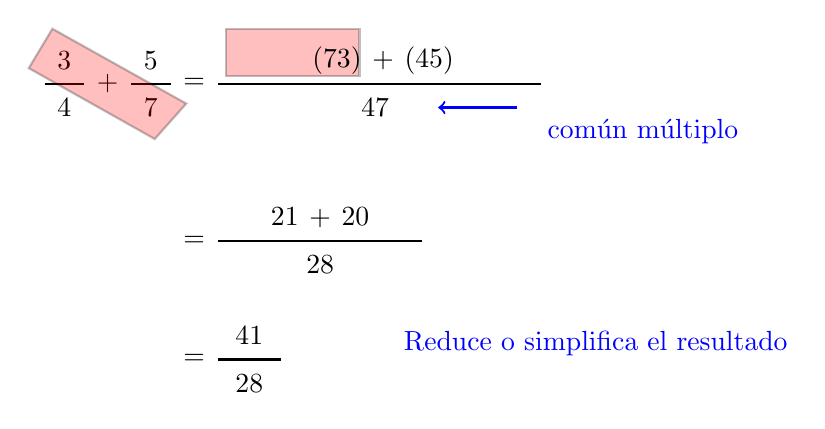
\begin{tikzpicture}[thick]
    \draw (0, 1) -- (0.5, 1);
    \node at (0.25, 1.3) {$3$};
    \node at (0.25, 0.7) {$4$};
    \node at (0.8, 1) {$+$};

    \draw (1.1, 1) -- (1.6, 1);
    \node at (1.35, 1.3) {$5$};
    \node at (1.35, 0.7) {$7$};
    \node at (1.9, 1) {$=$}; \pause

    \draw (2.2, 1) -- (6.3, 1);
    \node at (4.2, 0.7) {$4 \cp 7$};
    \draw [<-, thick, blue] (5, 0.7) -- (6, 0.7);
    \node [blue] at (7.6, 0.4) {común múltiplo}; \pause

    \draw [fill=red, opacity=0.25] (-0.2, 1.2) -- (1.4, 0.3) -- (1.8, 0.75) -- (0.1, 1.7) -- (-0.2, 1.2) -- cycle;

    \draw [fill=red, opacity=0.25] (2.3, 1.1) rectangle (4, 1.7);

    \node at (4.3, 1.3) {$(7 \cp 3) \, + \, (4 \cp 5)$}; \pause
    \node at (1.9, -1) {$=$};

    \draw (2.2, -1) -- (4.8, -1);

    \node at (3.5, -0.7) {$21 \, + \, 20$};
    \node at (3.5, -1.3) {$28$}; \pause

    \node at (1.9, -2.5) {$=$};

    \draw (2.2, -2.5) -- (3, -2.5);
    \node at (2.6, -2.2) {$41$};
    \node at (2.6, -2.8) {$28$};

    \node [text=blue] at (7, -2.3) {Reduce o simplifica el resultado};
\end{tikzpicture}
\end{figure}
\end{frame}
\begin{frame}
\frametitle{Ejemplo de una resta}
Veamos un ejemplo
\begin{figure}
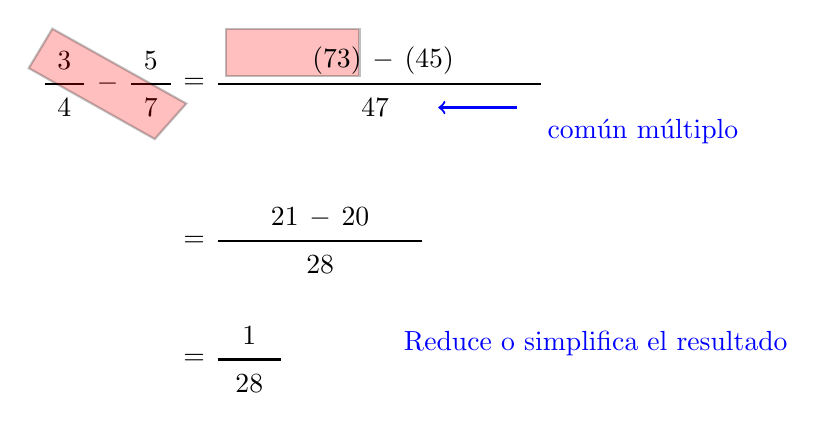
\begin{tikzpicture}[thick]
    \draw (0, 1) -- (0.5, 1);
    \node at (0.25, 1.3) {$3$};
    \node at (0.25, 0.7) {$4$};
    \node at (0.8, 1) {$-$};

    \draw (1.1, 1) -- (1.6, 1);
    \node at (1.35, 1.3) {$5$};
    \node at (1.35, 0.7) {$7$};
    \node at (1.9, 1) {$=$}; \pause

    \draw (2.2, 1) -- (6.3, 1);
    \node at (4.2, 0.7) {$4 \cp 7$};
    \draw [<-, thick, blue] (5, 0.7) -- (6, 0.7);
    \node [blue] at (7.6, 0.4) {común múltiplo}; \pause

    \draw [fill=red, opacity=0.25] (-0.2, 1.2) -- (1.4, 0.3) -- (1.8, 0.75) -- (0.1, 1.7) -- (-0.2, 1.2) -- cycle;

    \draw [fill=red, opacity=0.25] (2.3, 1.1) rectangle (4, 1.7);

    \node at (4.3, 1.3) {$(7 \cp 3) \, - \, (4 \cp 5)$}; \pause
    \node at (1.9, -1) {$=$};

    \draw (2.2, -1) -- (4.8, -1);

    \node at (3.5, -0.7) {$21 \, - \, 20$};
    \node at (3.5, -1.3) {$28$}; \pause

    \node at (1.9, -2.5) {$=$};

    \draw (2.2, -2.5) -- (3, -2.5);
    \node at (2.6, -2.2) {$1$};
    \node at (2.6, -2.8) {$28$};

    \node [text=blue] at (7, -2.3) {Reduce o simplifica el resultado};
\end{tikzpicture}
\end{figure}
\end{frame}
\begin{frame}
\frametitle{Ejemplo de una suma con tres fracciones}
Veamos un ejemplo
\begin{figure}
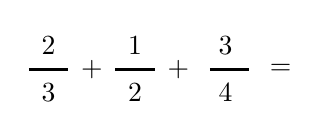
\begin{tikzpicture}[thick]
    \draw (0, 1) -- (0.5, 1);
    \node at (0.25, 1.3) {$2$};
    \node at (0.25, 0.7) {$3$};
    \node at (0.8, 1) {$+$};

    \draw (1.1, 1) -- (1.6, 1);
    \node at (1.35, 1.3) {$1$};
    \node at (1.35, 0.7) {$2$};
    \node at (1.9, 1) {$+$};

    \draw (2.3, 1) -- (2.8, 1);
    \node at (2.5, 1.3) {$3$};
    \node at (2.5, 0.7) {$4$};

    \node at (3.2, 1) {$=$};
\end{tikzpicture}
\end{figure}
\pause
Tenemos que encontrar el \textcolor{red}{mínimo común múltiplo}.
\begin{align*}
&2, \, 4, \, 6, \, 8, \, 10, \, {\color{red}{12}}, \, 14 \\[0.25em]
&3, \, 6, \, 9, \, {\color{red}{12}}, \, 15, \, 18, \, 21 \\[0.25em]
&4, \, 8, \, {\color{red}{12}}, \, 16, \, 20, \, 24, \, 28
\end{align*}
\end{frame}
\begin{frame}
\frametitle{Operación de la suma}
Una vez que hemos hallado el \textcolor{red}{m.c.m.}, ahora dividimos ese valor entre cada uno de los denominadores de las fracciones, el resultado lo multiplicamos por el numerador y lo acomodamos en una suma:
\end{frame}
\begin{frame}
\frametitle{Ejemplo de una suma con tres fracciones}
\begin{figure}
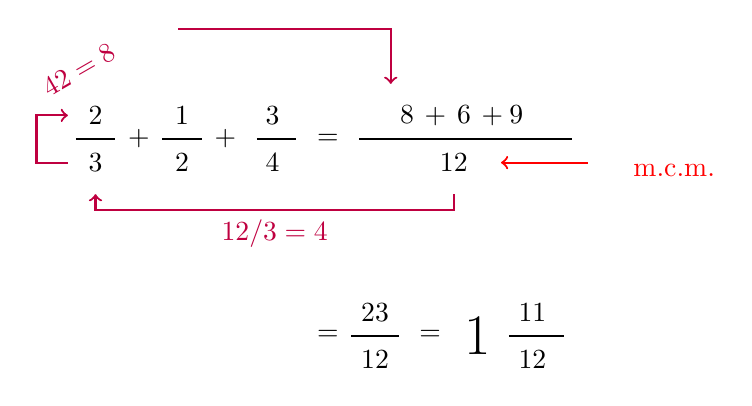
\begin{tikzpicture}[thick]
    \draw (0, 1) -- (0.5, 1);
    \node at (0.25, 1.3) {$2$};
    \node at (0.25, 0.7) {$3$};
    \node at (0.8, 1) {$+$};

    \draw (1.1, 1) -- (1.6, 1);
    \node at (1.35, 1.3) {$1$};
    \node at (1.35, 0.7) {$2$};
    \node at (1.9, 1) {$+$};

    \draw (2.3, 1) -- (2.8, 1);
    \node at (2.5, 1.3) {$3$};
    \node at (2.5, 0.7) {$4$};

    \node at (3.2, 1) {$=$}; \pause

    \draw (3.6, 1) -- (6.3, 1);
    \node at (4.8, 0.7) {$12$};
    \draw [<-, thick, red] (5.4, 0.7) -- (6.5, 0.7);
    \node [red] at (7.6, 0.6) {m.c.m.}; \pause

    \draw [purple, thick, ->] (4.8, 0.3) -- (4.8, 0.1) -- (0.25, 0.1) node [below, midway] {$12 / 3 = 4$} -- (0.25, 0.3); \pause

    \draw [purple, thick, ->] (-0.1, 0.7) -- (-0.5, 0.7) -- (-0.5, 1.3) -- (-0.1, 1.3);

    \node[text=purple, rotate around={30:(-0.1, 1.7)}] at (-0.8, 1.6) {$4 \cp 2 = 8$}; \pause

    \draw [->, purple] (1.3, 2.4) -- (4, 2.4) -- (4, 1.7);

    
    \node at (4.9, 1.3) {$8 \, + \, 6 \, + 9$}; \pause

    \node at (3.2, -1.5) {$=$};

    \draw (3.5, -1.5) -- (4.1, -1.5);

    \node at (3.8, -1.2) {$23$};
    \node at (3.8, -1.8) {$12$}; \pause

    \node at (4.5, -1.5) {$=$};

    \node at (5.1, -1.5) {\text{\huge $1$}};
    \draw (5.5, -1.5) -- (6.2, -1.5);
    \node at (5.8, -1.2) {$11$};
    \node at (5.8, -1.8) {$12$};
\end{tikzpicture}
\end{figure}
\end{frame}
\begin{frame}
\frametitle{Producto de fracciones}
Al multiplicar las fracciones:
\setbeamercolor{item projected}{bg=blue!70!black,fg=yellow}
\setbeamertemplate{enumerate items}[circle]
\begin{enumerate}[<+->]
\item Multiplicamos los numeradores, el valor que obtengamos, queda como numerador.
\item Multiplicamos los denominadores, el valor que obtengamos, queda como denominador.
\end{enumerate}
\end{frame}
\begin{frame}
\frametitle{Esquema de la multiplicación de fracciones}
Multiplicando dos fracciones:
\begin{align*}
\dfrac{a}{b} \cp \dfrac{c}{d} = \dfrac{a \cp c}{b \cp d}
\end{align*}
\\
\bigskip
\pause
Multiplicando tres fracciones:
\begin{align*}
\dfrac{e}{f} \cp \dfrac{g}{h} \cp \dfrac{i}{k} = \dfrac{e \cp g \cp i}{f \cp h \cp k} 
\end{align*}
\end{frame}
\begin{frame}
\frametitle{División entre fracciones}
La división entre fracciones sigue una regla que podemos esquematizar de la siguiente manera: hacemos productos (multiplicaciones) cruzados:
\begin{figure}
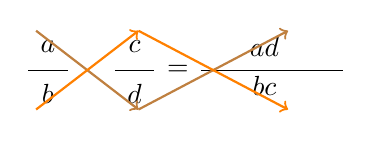
\begin{tikzpicture}
    \draw (0, 0.5) -- (0.5, 0.5);
    \node at (0.25, 0.8) {$a$};
    \node at (0.25, 0.2) {$b$};
    \node at (0.8, 0.5) {$\divisionsymbol$};
    \draw (1.1, 0.5) -- (1.6, 0.5);
    \node at (1.35, 0.8) {$c$};
    \node at (1.35, 0.2) {$d$};
    \node at (1.9, 0.5) {$=$};
    \draw (2.2, 0.5) -- (4, 0.5); \pause

    \draw [->, brown, thick] (0.1, 1) -- (1.4, 0); \pause
    \node at (3, 0.8) {$a \cp d$};
    \draw [->, brown, thick] (1.4, 0) -- (3.3, 1); \pause

    \draw [->, orange, thick] (0.1, 0) -- (1.4, 1); \pause

    \node at (3, 0.3) {$b \cp c$};
    \draw [->, orange, thick] (1.4, 1) -- (3.3, 0);
\end{tikzpicture}
\end{figure}
\end{frame}

\section{Ejercicios}
\frame{\tableofcontents[currentsection, hideothersubsections]}
\subsection{Operaciones con fracciones}

\begin{frame}
\frametitle{Resuelve y simplifica las siguiente operaciones}
\begin{table}
\renewcommand{\arraystretch}{2}
\begin{tabular}{l l}
$1).$ & $\dfrac{1}{2} - \dfrac{1}{6}$ \\
$2).$ & $\dfrac{3}{5} - \dfrac{1}{106}$ \\
$3).$ & $\dfrac{7}{12} - \dfrac{1}{4}$ \\
$4).$ & $\dfrac{11}{8} - \dfrac{7}{24}$ \\
\end{tabular}
\end{table}
\end{frame}
\begin{frame}
\frametitle{Resulve las siguientes operaciones mixtas}
\begin{table}
\renewcommand{\arraystretch}{2}
\begin{tabular}{l l}
$1).$ & $\dfrac{2}{3} + \dfrac{5}{6} - \dfrac{1}{12} $ \\
$2).$ & $\dfrac{3}{4} - \dfrac{5}{8} + \dfrac{7}{12}$ \\
$3).$ & $\dfrac{7}{12} + \dfrac{5}{9} - \dfrac{4}{24}$ \\
$4).$ & $\dfrac{11}{15} - \dfrac{7}{30} + \dfrac{3}{10}$ \\
\end{tabular}
\end{table}
  
\end{frame}
\end{document}